%-------------------------------------------------------------------------------
%	CAPITOLO 41
%-------------------------------------------------------------------------------

\chapter{I due Capelli - Gioti}
\index[Personaggi]{Capelli (avvocato)}Uno affogato nel vino. Parliamo di quello. Era un valore come legale, conscio del suo valore ne era altero e soffriva mal volentieri di fare il suo tirocinio alle dipendenze di un celebre avvocato di \index[Luoghi]{Bologna}Bologna il quale trionfava nei Tribunali con le difese del nostro uomo.\\
\indent L'applicazione allo studio, il mal trattamento od altro rovinarono la salute del nostro emerito avvocato... ed i genitori lo vollero a casa per guadagnare la salute.\\
\indent Qui era medico primario il povero dott. \index[Personaggi]{Gamberini Dr. Giulio}Gamberini, che aveva una grande fiducia nei buoni effetti rigenerativi del vino e cognac.\\
\indent Avendo sotto la sua casa il nostro avvocato, esile, allampanato... senza appetito ed astemio, cominciò a farlo trincare per rinvigorirlo. Fu una sbornia attaccata all'altra e lo rovinò.\\
\indent Solitamente la sbornia di carnevale cominciava in lui a Natale e finiva a Pasqua. Fiutava tabacco e chi lo avesse spolverato ne poteva ammassare qualche ettogrammo\footnote{Il protagonista era talmente impolverato che, scrollandolo, si poteva recuperare qualche ettogrammo di tabacco}.\\
\indent Il povero avvocato era ridotto ad uno stato miserevole dagli aiuti dell'alcool... in mezzo ad una festa da ballo, nella piazza affollata orinava in faccia al pubblico...\\
\indent Se la prendeva coi pretori perché non gli davano la vittoria nelle cause.\\

I suoi ritornelli ed invettive ai principali pretori, chi non li ricorda?
\textcal{	
\begin{center}
\Huge
No, anavoi Capolozzo! Capolozzo!\\
No, anavoi Mambrucon!\:\:\normalfont\normalsize\footnote{<<No, non voglio Capolozzo! Capolozzo; No, non voglio Mambrucone!>>}\footnote{Mambrucone fu pretore ad Alfonsine. Citando Romano Pasi: "Questo pretore Scognamiglio, principe meridionale, soffriva molto il freddo alfonsinese, per cui ascoltava le parti in causa standosene al calduccio del letto, mentre al cancelliere faceva mettere tutto agli atti. Quando la corte si ritirava per deliberare, si tirava la coperta sul capo, e dopo un po', scoprendo il volto, emetteva la sentenza."}
\end{center}}
\index[Personaggi]{Capolozzo}\index[Personaggi]{Mambrucone (pretore)}
\normalfont \normalsize
\noindent Di lui era caratteristica la macchietta.\\
Ecco l'uomo colto... ridotto incolto... dall'alcool.
 \begin{figure}[htb]
    \centering
    %\vspace{-0.7cm}
    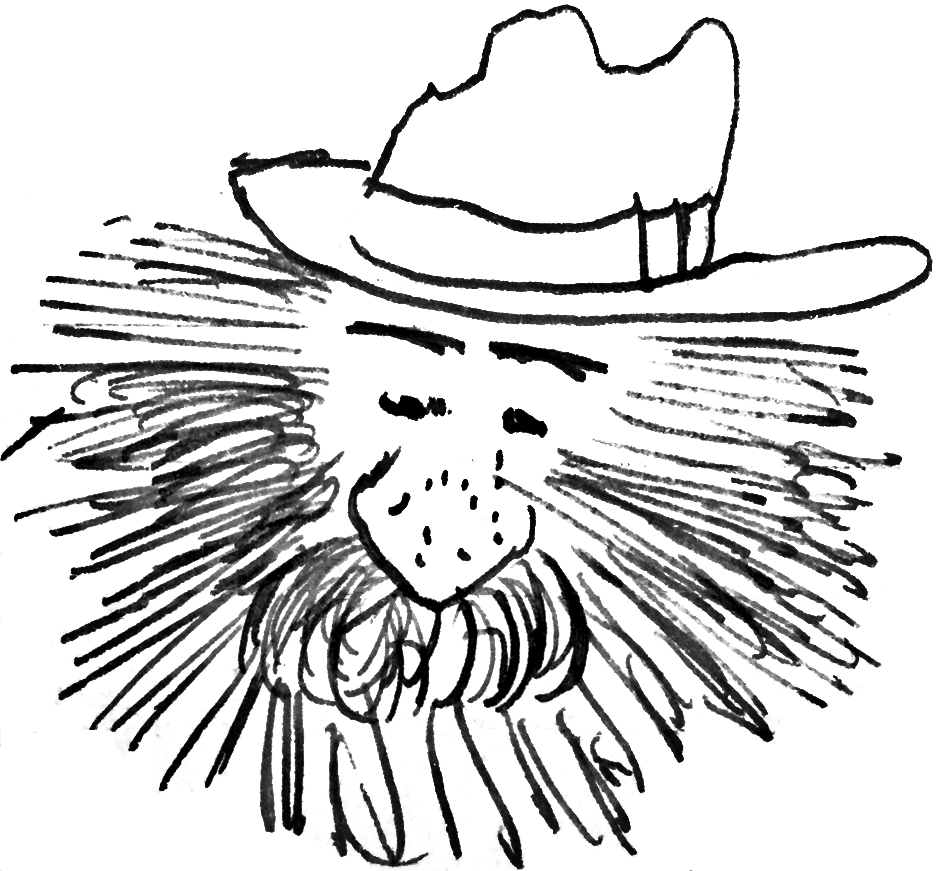
\includegraphics[height=6cm]{Capelli_Avvocato}
    %\vspace{-0.3cm}
\end{figure}\newpage
\index[Personaggi]{Capelli (protocollista)}

Sotto l'altro\footnote{E ora parliamo dell'altro}. \\Per questo la gola fu fatale. I tortelli hanno ucciso Capelli\footnote{Mia nonna Mariannina Gagliardi, nipote di Mingazzi, si ricorda che spesso Mingazzi raccontava di un certo "Zucò 'd Capèli", il protagonista di questa storiella.}, questa orrenda notizia vi dò!\\
\indent Tipo curioso, si credeva bello, irresistibile alle donne. Permaloso, un pò tardo di comprendonio sotto lo sforzo della digestione.\\
\indent Offriva a tutte le belle ragazze 100 scudi per una gita... con lui a \index[Luoghi]{Ravenna}Ravenna. Distribuiva a 60 anni, alle sue dame il suo ritratto all'età di 20 anni, vestito da sottotenente, nella sua caratteristica figura. La faccia sembrava una gran luna con sopra un guscio d'ovo, che era il berretto, due baffetti spioventi alla cinese, occhini coperti da grosse palpebre, sembrava un maiale della grassa. \\
\indent Si riteneva molto eloquente, faceva il causidico\footnote{Avvocato da poco, di bassa lega.} in pretura ed una volta presentò una comparsa con citazioni latine... che non conosceva. Il Pretore \index[Personaggi]{De Simone (pretore)}De Simone, ebbe a dirgli: <<Ecco spieghi questa...>>\\
\indent Al nostro causidico cadde il mondo addosso e credè rispondere: <<Ecco... si... già... s'intende...>> e fu una risata generale.\\
\indent Aveva lo stipendio da protocollista in comune, ma il suo tempo era diviso per le seguenti funzioni:\\
\begin{itemize}
\item[9.00]purga con acqua - Janos\footnote{Acqua medicinale Hunyadi János, conosciuta e consumata dal 1863, costituita da sale di Glauber e sale inglese.}
\item[10.00]leggere sotto lo scaffale della scrivania il giornale, e brontolare a chi osava varcare la porta del suo ufficio: <<Ho da fare lasciatemi in pace...>>
\item[11.00]entrata nella vecchia latrina del palazzo comunale, dove c'era una gran pietra per posare i piedi, dietro una buca di m. 1,50 per 0,80 e dopo il muro.\\
Giù le brache... chino il corpo in orizzontale, non arrivava ad accovacciarsi sui polpacci... che la scarica avveniva nel muro di contro con una rosa di almeno 60 centimetri. \\
Chi andava dopo di lui vedeva i segni di \index[Personaggi]{Capelli (protocollista)}Capelli.
\item[11.30]Andava alla firma, riceveva 4,5 lettere da protocollare.
\item[12.00] a mangiare.
\item[13.00] a fare il chilo sul sofà e respirare a due riprese, perché troppo pieno.
\item[13.30] per la strada presso le fruttivendole a mangiare arance, mele, mandarini, zucca cotta ecc.
\item[14.00] all'ufficio a cominciare missive d'affari sui grandi fogli da protocollo, poi accartocciava tutto... perché sbagliava perché era troppo pieno... e non concepiva il pensiero.
\item[17.00] (d'inverno) uscito dall'ufficio, passava a rifornirsi di cioccolatini e poi da qualche bella a farseli mangiare.
\item[18.00](se d'estate) all'osteria a ordinare un etto di mortadella, o salame, mezzo litro di vino, e due soldi di pane, con molti bis.
\item[19 - 20] a cena a divorar tutto.
\item[20.30] al caffè cominciava a bere latte mangiar paste, biscotti, pan di Spagna ecc. per qualche mezzo chilo.
\item[21.30] a morosa fino alle 22
\item[22.00] entrato nell'osteria annusava come un cane da trifola, poi chiedeva : <<Che cosa hai rimasto?>>\\
\indent Oste: <<Cappelletti, umido, arrosto, lesso."\\
\indent \index[Personaggi]{Capelli (protocollista)}Capelli: <<Fammi vedere>> poi <<Quanto vuoi per tutto?>>\\
\indent Il contratto era fatto e tutto divorato.
\item[23.00] Chiudevano l'osteria ed il nostro uomo prendeva la via dell'amata... fino all'una.. a fare il chilo e farsi far vento alla pancia perché gli tirava per avere troppo mangiato...
\item[1.00] tornava a casa e dava aria ai polmoni... ed alla strada... per sgonfiare la pancia. Poi a letto fino alle 8.
\end{itemize}

Era assiduo di tutti gli spettacoli ai quali assisteva divorandosi brustole\footnote{Semi di zucca}, caramelle, cioccolatini ecc.\\
\indent Credeva di conquistare le commedianti o cantanti, ronzando sempre loro intorno come un molesto bagarone\footnote{Calabrone}.\\
\indent Una sera il pover'uomo era a godersi uno spettacolo, seduto su una delle prime fila di sinistra del \index[Luoghi]{Teatro Calderoni, Baraccone}Baraccone. Aveva mangiato più del solito, la sua testa era in confusione credendosi ammirato... (e per questo era abile perché aveva una gran cura di mostrare alle artiste il portafoglio e di promettere molto...) ma la digestione lo disturbava molto e lo assopiva. Però non poteva né assopirsi né sedersi comodamente... era come sugli spini per la gonfiezza.\\
\indent Sulla fine di un atto uscì, si appressò alla siepe del \index[Luoghi]{Carraretto Venturi}Carraretto\footnote{Carraretto Venturi, il teatro Baraccone fu spostato nel Carraretto Venturi (e lazarètt) già dal 1894}, ad orinare quando credé di fare uno sforzo per vuotare l'aria... ma il colpo fu tale e forte... da prendere una lombaggine\footnote{Dolore in sede lombare che si acutizza nei movimenti di flessione ed estensione del tronco} (snestar\footnote{Espressione dialettale per `colpo della strega'}) e dovettero portarlo a casa, e chiamato il povero \index[Personaggi]{Novi (dottore)}Dr. Novi e l'infermiere \index[Personaggi]{Domenico Soatti `Mingò d'Galèna` (infermiere)}Mingone di Gallina\footnote{\textbf{Domenico Soatti}, detto Mingò d'Galèna,infermiere.}, che lo sottoposero ad una iniezione calmante.\\

\indent Era sempre tutto gentile... per non far torto al suo budello che tanto lo aiutava. Era geloso di tutti e di tutte.\\
\indent Il povero \index[Personaggi]{Isani Nando (farmacista)}Nando Isani, aiuto farmacista da \index[Personaggi]{Boari Attilio (farmacista)}Boari, quando lo vedeva venire serrava la bussola\footnote{Portantina} della farmacia e si nascondeva nel laboratorio.\\
\indent Cominciava allora la scena da ridere. \index[Personaggi]{Capelli (protocollista)}Capelli, spingeva la bussola, chiamava... strimpellava, perché si metteva in sospetto che nel retro farmacia Nando \index[Personaggi]{Isani Nando (farmacista)} avesse qualche avventura galante... e lui voleva sorprenderlo... per intimare alla femmina... amore anche per lui... \\
\indent La porta rimaneva chiusa e \index[Personaggi]{Capelli (protocollista)}Capelli guardia portone, finché dopo un gran pezzo appariva il povero Nando \index[Personaggi]{Isani Nando (farmacista)} facendo l'imbronciato, e cominciava il dialogo.\\
\indent Capelli: <<Chi avevi...>>\\
\indent Nando: <<Nessuno, che cosa vuol sapere!>>\\
\indent Capelli: <<Va là dimmelo, ti vuoi godere solo tu... ed insisteva per delle ore...>>\\
\indent Capelli a qualche altro: <<Mo chi era la donna, dove è?>>\\
\indent Interrogato: <<Stia zitto è scappata dalla porta di dietro!>>\\
\indent Capelli: <<Porca, non sono capace di trovarla!>>\\
\indent E la commedia si ripeteva spesso... tra le risate.\\

\indent Una delle sue amate stava in \index[Luoghi]{Vincenzo Monti (piazza)}Piazza\footnote{Piazza Monti} di fronte al \index[Luoghi]{Palazzo Comunale}Palazzo Comunale ed aveva le finestre al 2\textsuperscript{o} piano.\\
\indent \index[Personaggi]{Capelli (protocollista)}Capelli si metteva alla finestra del \index[Luoghi]{Palazzo Comunale}Palazzo Comunale, la sua amata... alla sua, distante 150 metri e pretendeva di essere ammirato. Una volta poi avvenne che i saltimbanchi eressero in \index[Luoghi]{Vincenzo Monti (piazza)}Piazza grandi tende ed impedirono l'idillio di ammirazione. Il nostro \index[Personaggi]{Capelli (protocollista)}Capelli se la prese con l'amata... e la piantò per qualche tempo.\\
\indent L'amata però mal soffriva un tale ingiusto trattamento e decise di fermare l'amato bene un sera quando andava a casa. Il colloquio si svolse così:\\
\indent Amata: <<Perché non vieni più?>>\\
\indent Capelli: <<Perché non mi hai guardato dalla finestra...>>\\
\indent Amata: <<Ma come devo fare, ci sono le baracche in mezzo e non si può vedere...>>\\
\indent Capelli: <<A na voi savé me, va dsò da la Pia... (al 3\textsuperscript{o} piano) me a voi t'am guerda\footnote{<<Non lo voglio sapere io, va di sopra dalla Pia, io voglio che tu mi guardi>>}>>.\\

\newpage
Ammiriamo anche noi questo pachiderma.
 \begin{figure}[htb]
    \centering
    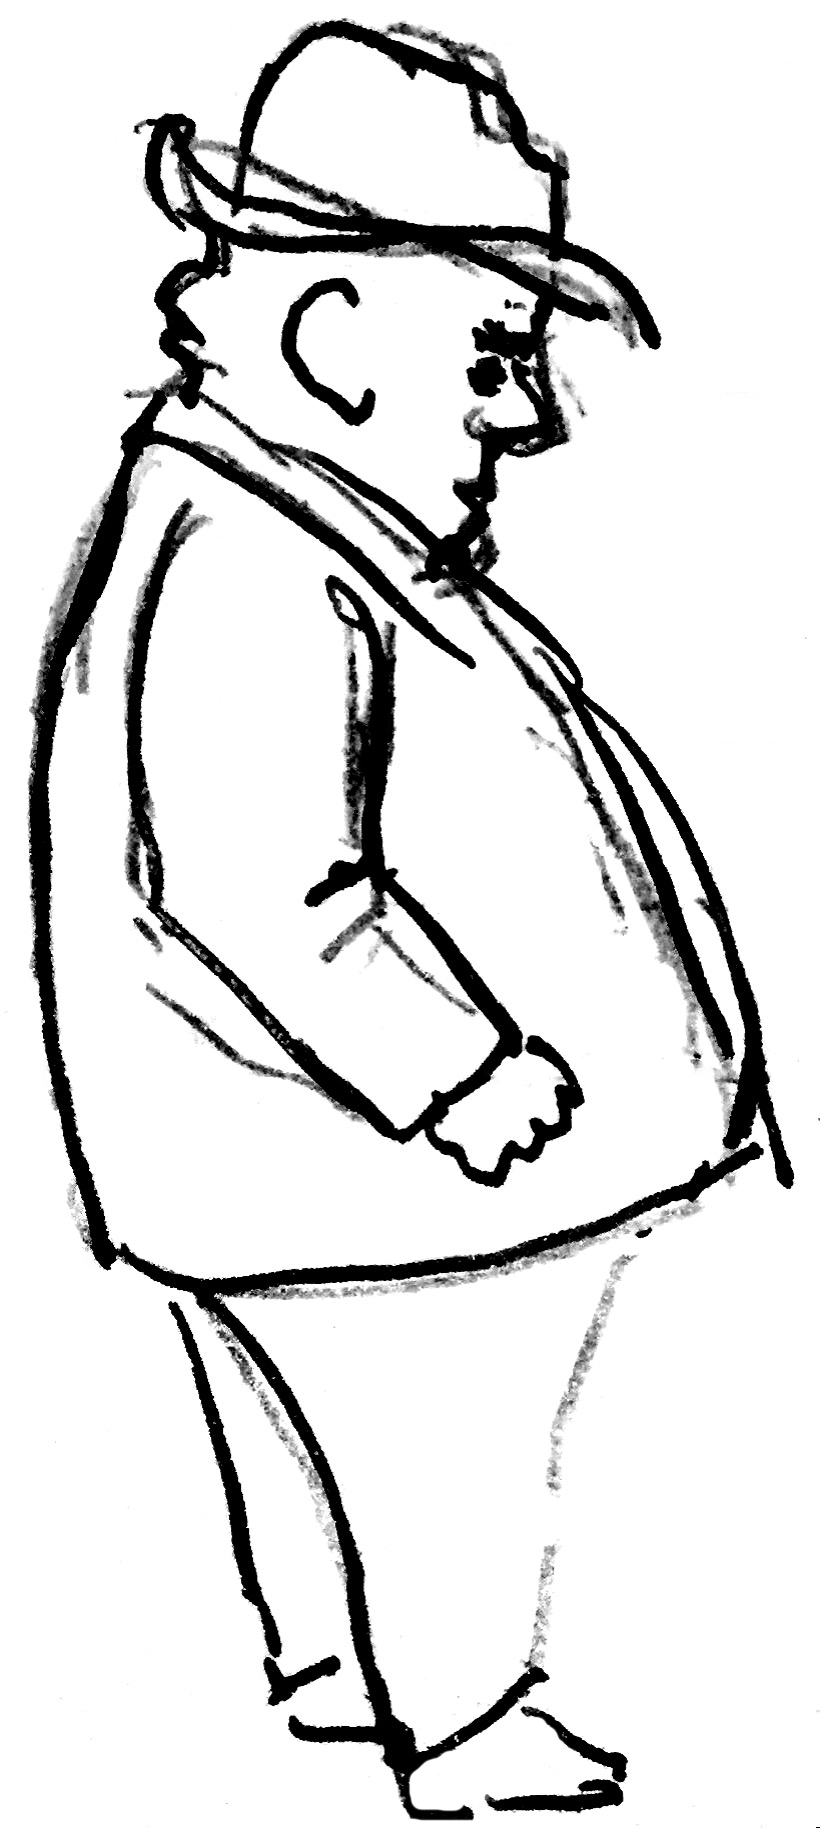
\includegraphics[width=0.6\textwidth]{Capelli_mangione}
    %\vspace{-0.3cm}
\end{figure}

\newpage
\indent Teneva regalare copia e minute\footnote{Le prime stesure provvisorie delle lettere} delle lettere amorose che riceveva, la collezione dei ricciolini... e di altri peli ancor più fini...\\
\indent Dopo morto si trovò tutto questo materiale documentario della sua attività conquistatrice ed una cambiale, con la firma del povero \index[Personaggi]{Capelli (protocollista)}Capelli ed altra persona con accompagnato un biglietto così concepito:
\begin{center}
	\emph{Caro Capelli, vi mando la cambiale che avete firmato per me, che ho pagato, e che ora ha solo un valore di riconoscenza. Vi prego di distruggerla, perché se la trovano i vostri eredi diranno che vi siete mangiati anche quelli...}
\end{center}

 \begin{figure}[htb]
    \centering
    %\vspace{-0.7cm}
    \includegraphics[width=\textwidth]{mingò}
    \caption*{L'uomo con gli occhiali seduto al centro è \textbf{Domenico Soatti}, "Mingò 'd Galèna"\index[Personaggi]{Domenico Soatti `Mingò d'Galèna` (infermiere)}, mentre i due uomini in piedi sulla destra, partendo da sinistra sono: Stefano Mingazzi e \index[Personaggi]{Isani Nando}Nando Isani\label{fig:mingò}}
    %\vspace{-0.3cm}
\end{figure}

\newpage
\subsection{Gioti}
Questo capitoletto è presente nell'indice, ma non fu mai scritto. Questo è ciò che ho trovato nel quaderno:\\
\begin{figure}[!htbp]
   \includegraphics[width=\textwidth]{"Gioti".jpg}
\end{figure}
\\Probabilmente Mingazzi voleva scrivevere qualche racconto su \index[Personaggi]{Marchiani Luigi `Gioti'}Marchiani Luigi (08/06/1872 - 29/04/1934). Alcuni vecchi del paese ancora lo ricordano, sempre a spasso con il suo asinello.
\newpage
Riporto la prima pagina del racconto su Gioti della mia cara amica \index[Personaggi]{Forlivesi Edda}Edda Forlivesi.\\

 \begin{figure}[htb]
    \centering
    %\vspace{-0.7cm}
    \includegraphics[width=\textwidth]{Gioti2}
    %\vspace{-0.3cm}
\end{figure}

\noindent \textit{Traduzione}: Gioti stava nella casa dei Zalambani, quella che hanno buttato giù; là c'era il circolo, e sotto al circolo di Vincenzo Monti, c'era Gioti, e lì in tutta quanta la casa vecchia, comandava Bosi di Lugo. È stato 42 anni lì e non ha mai pagato l'affitto un anno. Un bel giorno arriva Bosi di Lugo e gli dice: <<Ciò, Marchiani (lui si chiamava Marchiani) qui...>> (lui faceva il sarto e la mattina prendeva il somaro che lo chiamava `Girardengo', e poi andava a contadini. Tornava a casa la sera, come al solito, sempre ubriaco).\\
\indent E una mattina arriva Bosi, lui è lì che prende il somaro e gli fa:\\
\indent <<Ciò Marchiani, qui se non paghi l'affitto, sono costretto a mandarvi via da qui!>>\\
\indent <<Eccolo, finisco di mettere le redini al somaro e poi me ne vado subito!>>\\
\indent <<No, No, qui, o comprate oppure ve ne andate!>>\\
\indent <<Io pensavo di vendere>> gli rispose Gioti.\\



























